\documentclass[15pt,a5paper,reqno]{article}
\usepackage{hyperref}
\usepackage[warn]{mathtext}
\usepackage[utf8]{inputenc}
\usepackage[T2A]{fontenc}
\usepackage[russian]{babel}
\usepackage{amssymb, amsmath, multicol}
\usepackage{graphicx}
\usepackage[shortcuts,cyremdash]{extdash}
\usepackage{wrapfig}
\usepackage{floatflt}
\usepackage{lipsum}
\usepackage{verbatim}
\usepackage{concmath}
\usepackage{euler}
\usepackage{xcolor}
\usepackage{etoolbox}
\usepackage{fancyhdr}
\usepackage{subfiles}
\usepackage{enumitem}
\usepackage{amsthm}
\usepackage{indentfirst}
\usepackage{import}

\DeclareMathOperator{\sign}{sign}

\RequirePackage[ left     = 1.5cm,
  right    = 1.5cm,
  top      = 2.0cm,
  bottom   = 1.25cm,
  includefoot,
  footskip = 1.25cm ]{geometry}
\setlength    {\parskip}        { .5em plus .15em minus .08em }
%\setlength    {\parindent}      { .0em }
\renewcommand {\baselinestretch}{ 1.07 }

\fancyhf{}

\renewcommand{\footrulewidth}{ .0em }
\fancyfoot[C]{\texttt{\textemdash~\thepage~\textemdash}}
\fancyhead[R]{\hfilШурыгин}

\makeatletter
\patchcmd\l@section{%
  \nobreak\hfil\nobreak
}{%
  \nobreak
  \leaders\hbox{%
    $\m@th \mkern \@dotsep mu\hbox{.}\mkern \@dotsep mu$%
  }%
  \hfill
  \nobreak
}{}{\errmessage{\noexpand\l@section could not be patched}}
\makeatother
\parindent = 1cm % отступ при красной строке⏎
\pagestyle{fancy}    
\renewcommand\qedsymbol{$\blacksquare$}

\newcommand{\when}[2]{
  \left. #1 \right|_{#2} \hspace
}
\renewcommand{\kappa}{\varkappa}
\RequirePackage{caption2}
\renewcommand\captionlabeldelim{}
\newcommand*{\hm}[1]{#1\nobreak\discretionary{}

\DeclareSymbolFont{T2Aletters}{T2A}{cmr}{m}{it}
{\hbox{$\mathsurround=0pt #1$}}{}}
% Цвета для гиперссылок
\definecolor{linkcolor}{HTML}{000000} % цвет ссылок
\definecolor{urlcolor}{HTML}{799B03} % цвет гиперссылок
 
\hypersetup{pdfstartview=FitH,  linkcolor=linkcolor,urlcolor=urlcolor, colorlinks=true}


\begin{document}
  
% НАЧАЛО ТИТУЛЬНОГО ЛИСТА

\begin{titlepage}
	\begin{center}
		\large 	Московский физико-технический университет \\
		Физтех-школа радиотехники и компьютерных технологий\\
		\vspace{0.2cm}
		
		\vspace{4.5cm}
		Лабораторная работа № 3.2.2 \\ \vspace{0.2cm}
		\LARGE \textbf{Резонанс напряжения в электрическом контуре}
	\end{center}
	\vspace{2.3cm} \large
	
	\begin{center}
		Работу выполнил: \\
		Шурыгин Антон \\
		Б01-909

	\end{center}
	
	\begin{center} \vspace{60mm}
		г. Долгопрудный \\
	\end{center}
\end{titlepage}

\textbf{Цель работы:}
Изучение явления саморепродукции и применение его к измерению параметров периодических структур.

\textbf{Оборудование:} лазер,кассета с сетками, мира, короткофокусная линза с микрометрическим винтом, экран, линейка.

\section{Введение и краткая теория}

    В работе предлагается измерить фокусные расстояния линз, смоделировать трубу Кеплера, трубу Галилея
    микроскоп и определить их увеличения.
    \newline

    \textbf{Сложенин центрированных оптических систем}
    Пусть две центрированные системы имеют общую главную оптическую ось. Если известны параметры каждой системы, а также их взаимное расположение, то аналитическим расчётом или геометрическим
    построением можно определить положение всех кардинальных точек
    сложной оптической системы, состоящей из этих двух систем.

    Рассматриваемая система схематически изображена на рис. 1.3.
    Кардинальные точки первой и второй систем отмечены соответствующими нижними индексами. Штрихами выделены кардинальные точки
    пространства изображений первой системы и аналогичные точки пространства предметов второй системы. 
    Величина $\Delta = F2 - F'1$ представляет расстояние от заднего фокуса первой системы до переднего фокуса
    второй системы и называется оптическим интервалом двух систем. 
    В соответствии с принятым правилом знаков $\Delta > 0$, если падающий светидёт от фокуса $F'1$ к фокусу $F2$, как отмечено стрелкой на рис. 1.3, в
    противоположном случае $\Delta < 0$. Заданием оптического интервала полностью определяется взаимное расположение складываемых систем.

    \begin{figure}[h!]
        \centering
        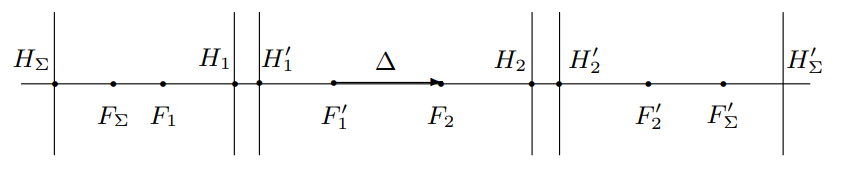
\includegraphics[width=0.8\linewidth]{pics/system_of_lens.png}
        \caption{Сложение центрированных систем}
        \label{}
    \end{figure}


    Конечные уравнения для фокусного расстояния и координат фокальных и главных точек сложной системы:


    \begin{equation}\label{1}
        f_{\sum} = - \frac{f_1 f_2}{\Delta}
    \end{equation}


    \begin{equation}\label{2}
        f'_{\sum } = - \frac{f'_1 f'_2}{\Delta}
    \end{equation}

    \begin{equation}\label{3}
        \Phi = \frac{n}{f_{\sum}} = -\frac{n\Delta}{f_1 f_2}
    \end{equation}



    \textbf{Примеры центрированных оптических систем}
    Оптическая система может не иметь фокальных плоскостей. Такая система называется афокальной или телескопической.
    Она является предельным случаем обычной системы, у которой фокальные плоскости сдвинуты в беконечность.
    Как видно из формул для сложных систем, телескопической становится система из двух обычных систем, если их оптический интервал $\Delta \rightarrow 0$

    Выполнив этот предельный переход в уравнениях, получим формулы для преобразования координат и коэффициенты увеличений телескопической системы:

    \[ \frac{x'}{x} = \frac{\delta x'}{\delta x} = \frac{f_2 f'_2}{f_1 f'_1} \]
    \[ \frac{y'}{y} = \frac{n \alpha}{n' \alpha'} = \frac{f_2}{f'_1} \]
    

    Из выражений выше следует, что в телескопической системе:
    \begin{enumerate}
        \item всякий параллельный пучок света после прохождения через систему остаётся параллельным
        \item продольное, поперечное и угловое увеличения постоянны, то есть не зависят от положения предмета.
    \end{enumerate}

    Оптическая сила телескопической системы, как видно из формулы \ref{3}, равна нулю.


\section{Схема установки}

\begin{figure}[h!]
    \centering
    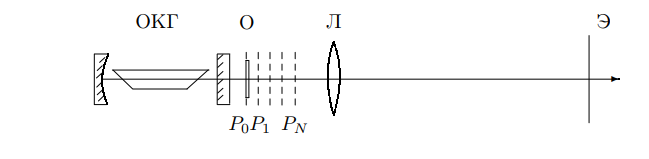
\includegraphics[width=15cm]{pics/scheme.png}
    \caption{Схема лабораторной установки}
    \label{fig:vac}
\end{figure}

\section{Ход работы}


\subsection{Измерение периода решеток по их пространственному спектру}


\begin{table}[h!]
	\centering
	\begin{tabular}{| c | c | c | c | c | c |}
    \hline
    $n_{сетки}$ & $X_m$, мм & $m$ & $x$, мм  & $d$, мм & $\sigma_d$, мм\\
    \hline
    1 & 201  & 6 & 33.50  &  0.020 & <0.001\\
    \hline
    2 & 223 & 9 & 24.77  &   0.027 & <0.001\\
    \hline
    3 & 177  & 16 & 11.1 &   0.061 & 0.001\\
    \hline
    4 & 235  & 24 & 9.79   &  0.069 & 0.001\\
    \hline
    5 & 63  & 16 & 3.93    &   0.174  & 0.007\\
    \hline
    \end{tabular}
    
	\caption{Измерение расстояние между соседними дифр. макс. на экране}
	\label{nu1}
\end{table}


Расстояние от кассеты до экрана $L = 124 \: cm$, $\lambda = 560 \: nm$.

\begin{equation}
    dsin(\theta_x) = m_x \lambda, \:\:\:\: d sin(\theta_y) = m_y \lambda     
  \label{first}
\end{equation}

Полагая $sin(\theta) \backsimeq \theta \backsimeq \frac{x}{L}$, найдем с помощью формул (1) период каждой решетки.

\[     d = \frac{\lambda L}{x}        \]

Измерения и результаты вычисления периоды дифракционной решетки занесены в таблицу 1.



\subsection{Измерение периода решеток по изображению, увеличенного с помощью линзы}

Найдем период решетки другим способом.
 
\begin{table}[h!]
	\centering
	\begin{tabular}{| c | c | c | c | c |}
\hline
$n_сетки$ & $x_m, mm$ & $m$ & $D, mm$ & $d, mm$\\
\hline
1 & - & - & - & -\\
\hline
2 & 3,5 & 6 & 0,58 & 0,027 \\
\hline
3 & 9 & 6 & 1,5 & 0,072\\
\hline
4 & 12 & 4 & 3 & 0,144\\
\hline
5 & 16 & 4 & 4 &  0,192\\
\hline
\end{tabular}

	\caption{Определение размера клеток $D$}
	\label{tb3}
\end{table}


Измеренные расстояния: между сеткой и экраном - $a' = 131 \: cm \rightarrow$ между линзой и сеткой -  $a = a' - b = 6 \: cm$ , между линзой и экраном - $ b= 125\:cm$.

\[    d = \frac{a}{b} \cdot D   \]

Таким образом по формуле выше находим период решетки и записываем результат в таблицу 2. 


\subsection{Исследование саморепродукции с помощью сеток}

Исследуем саморепродукцию.
Находим координаты $z_n$ плоскостей саморепродукции, строим график. По коэффициенту наклона прямой графика определим период решетки по формуле:

\begin{equation}
  d_i = \sqrt{\frac{k_i\lambda}{2}}
\end{equation}


\begin{table}[h!]
	\centering
	\begin{tabular}{| c | c | c | c | c | c |}
    \hline
          & $z_3, mm$ & $z_4, mm$  & $z_5, mm$\\
    \hline
        1 & - & 4 & 8,1 & 6,4 & 21,5\\
    \hline
        2 & - & 8,55 & 15,1 & 22,1 & 43,5\\
    \hline
        3 & - & 12,2 & 22 & 33,2 & 65,5\\
    \hline
        4 & - & 17,55 & 28,5 & 49,2 & -\\
    \hline
        5 & - & 20,55 & 35,2 & 59,7 & -\\
    \hline
        6 & - & 23,6 & 42 & - & -\\
    \hline
        7 & - & 28,8 & 49 & - & -\\
    \hline
        8 & - & - & 55,5 & - & -\\
  \hline
  \end{tabular}

	\caption{Измерение номера дифракционной картины от координаты линзы}
	\label{tb1}
\end{table}

\begin{table}[h!]
	\centering
	\begin{tabular}{| c | c | c | c | c | c |}
    \hline
    $n_сетки$ & 1 & 2 & 3 & 4 & 5  \\
    \hline
    $d, mm$   & - & 0,034 & 0,043 & 0,061 & 0,077   \\
    \hline
\end{tabular}
	\caption{Резульаты вычисления периода дифракционных решеток}
	\label{tb2}
\end{table}

Измерения и полученные значения сводим в таблицу 3. 
Затем строим графики $z = f(n)$.


\begin{figure}[h!]
  \centering
  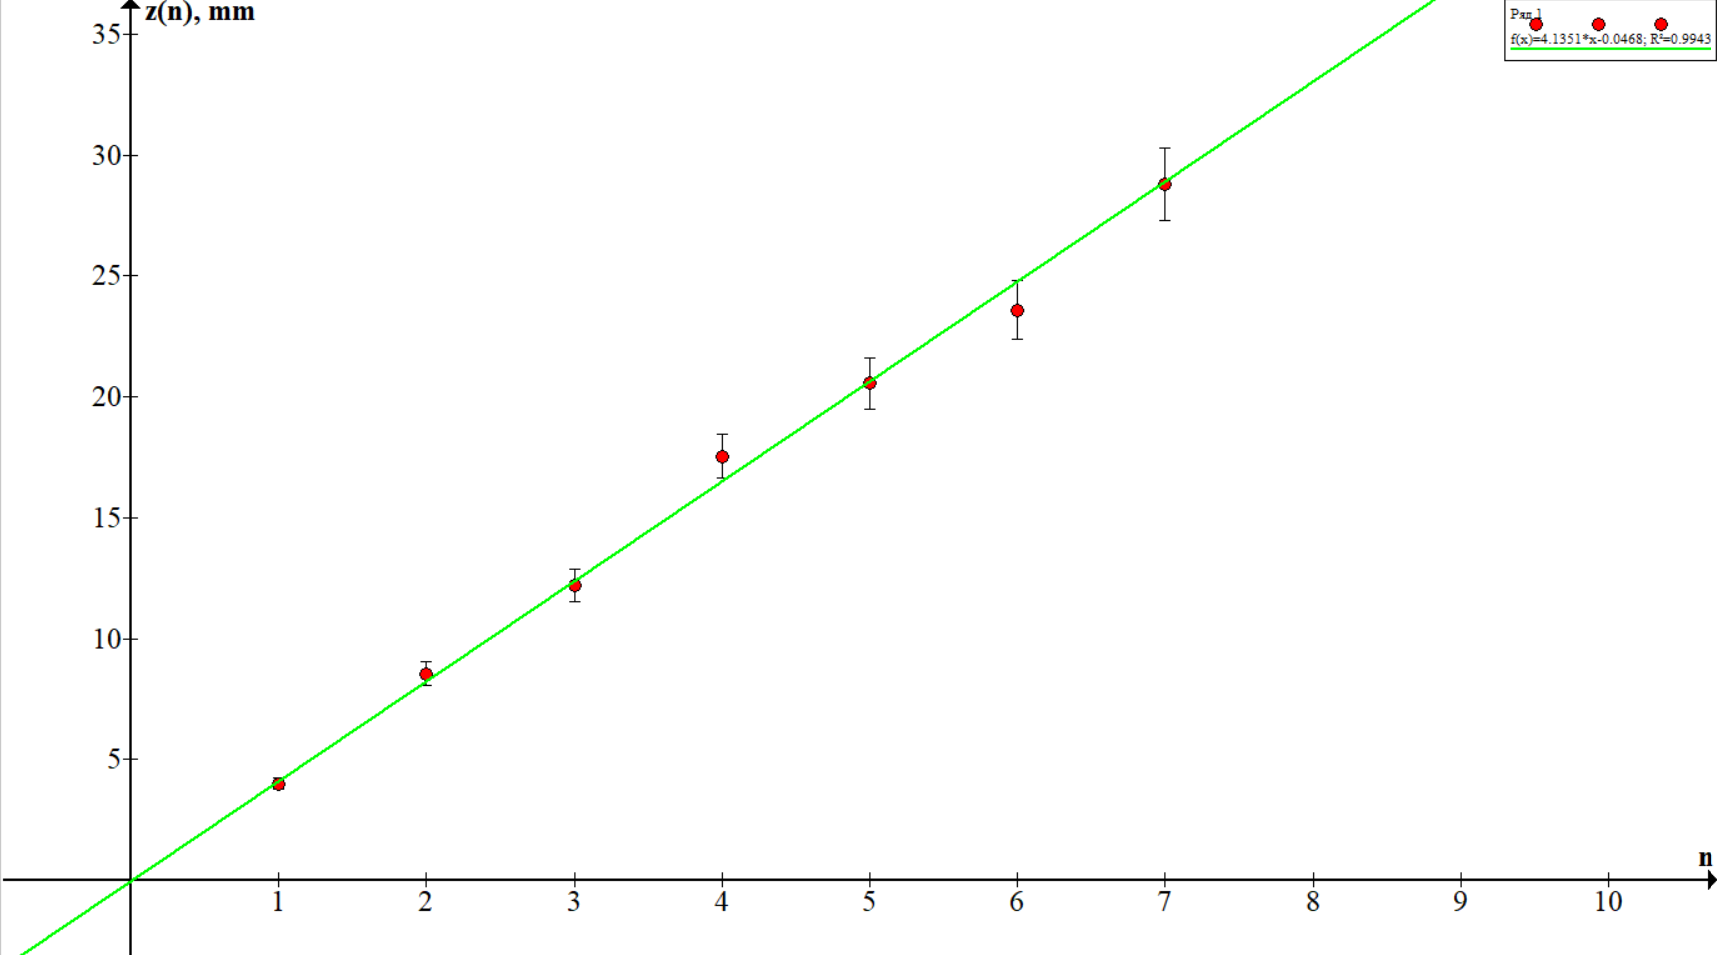
\includegraphics[width=13cm]{pics/lab_436_1.png}
  \caption{График $z_1 = f(n)$}
  \label{}
\end{figure}

\begin{figure}[h!]
  \centering
  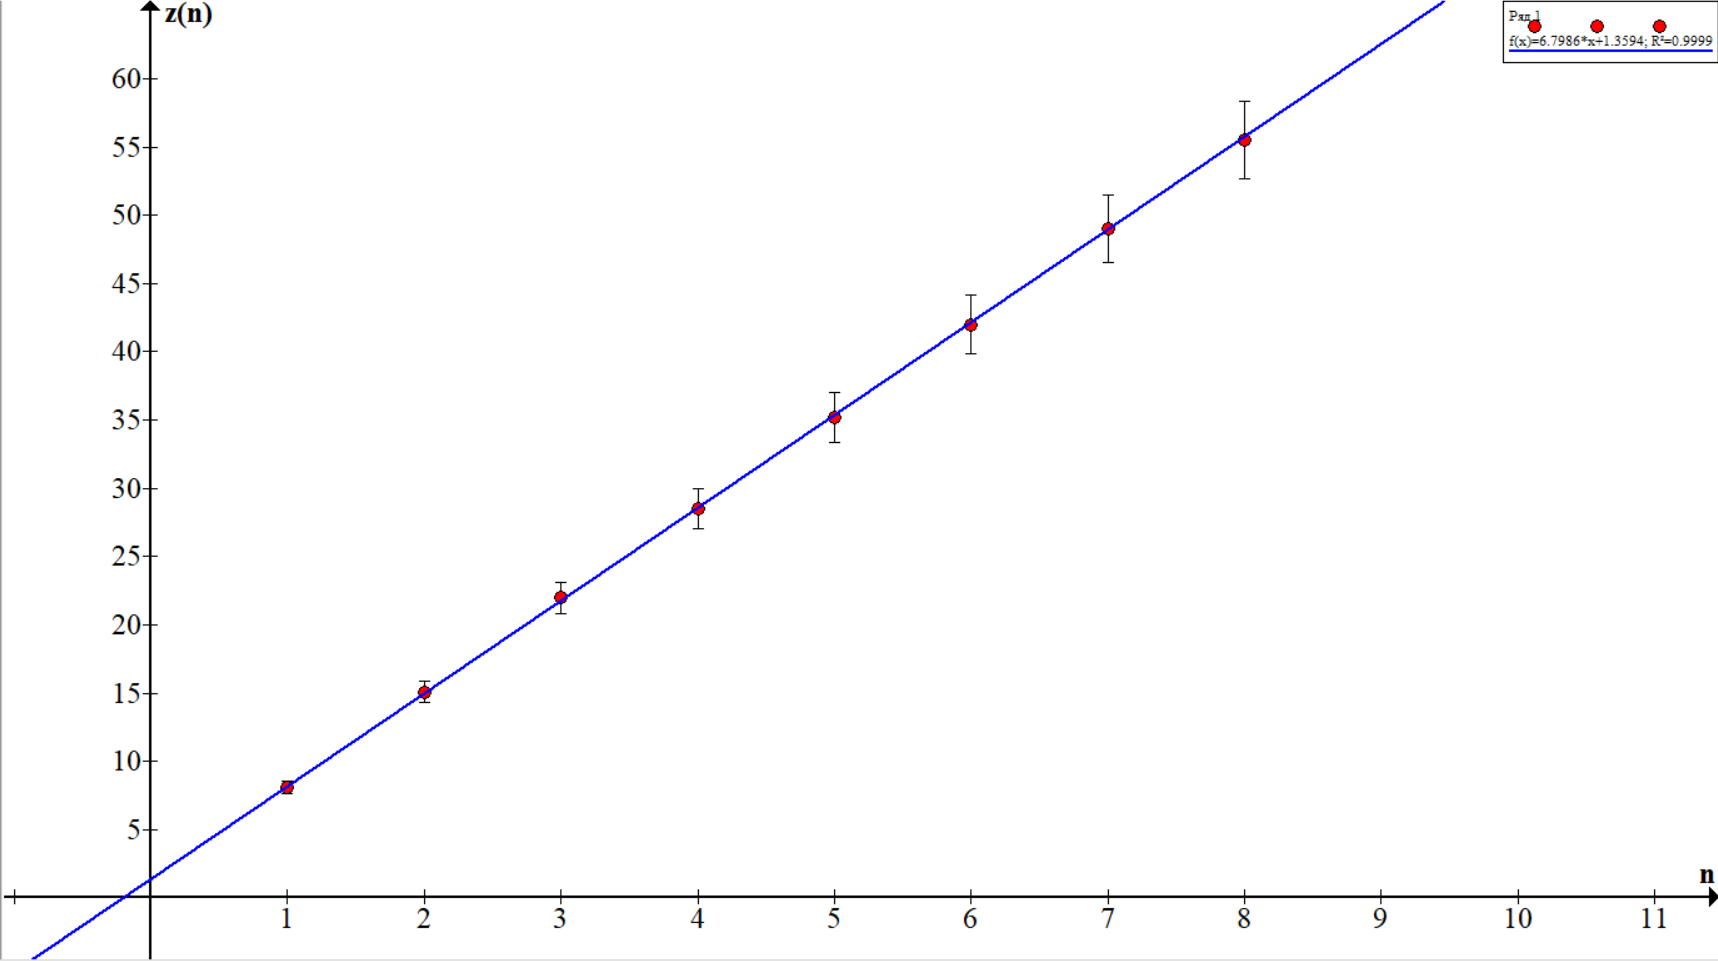
\includegraphics[width=13cm]{pics/lab_436_2.png}
  \caption{График $z_2 = f(n)$}
  \label{}
\end{figure}


\begin{figure}[h!]
  \centering
  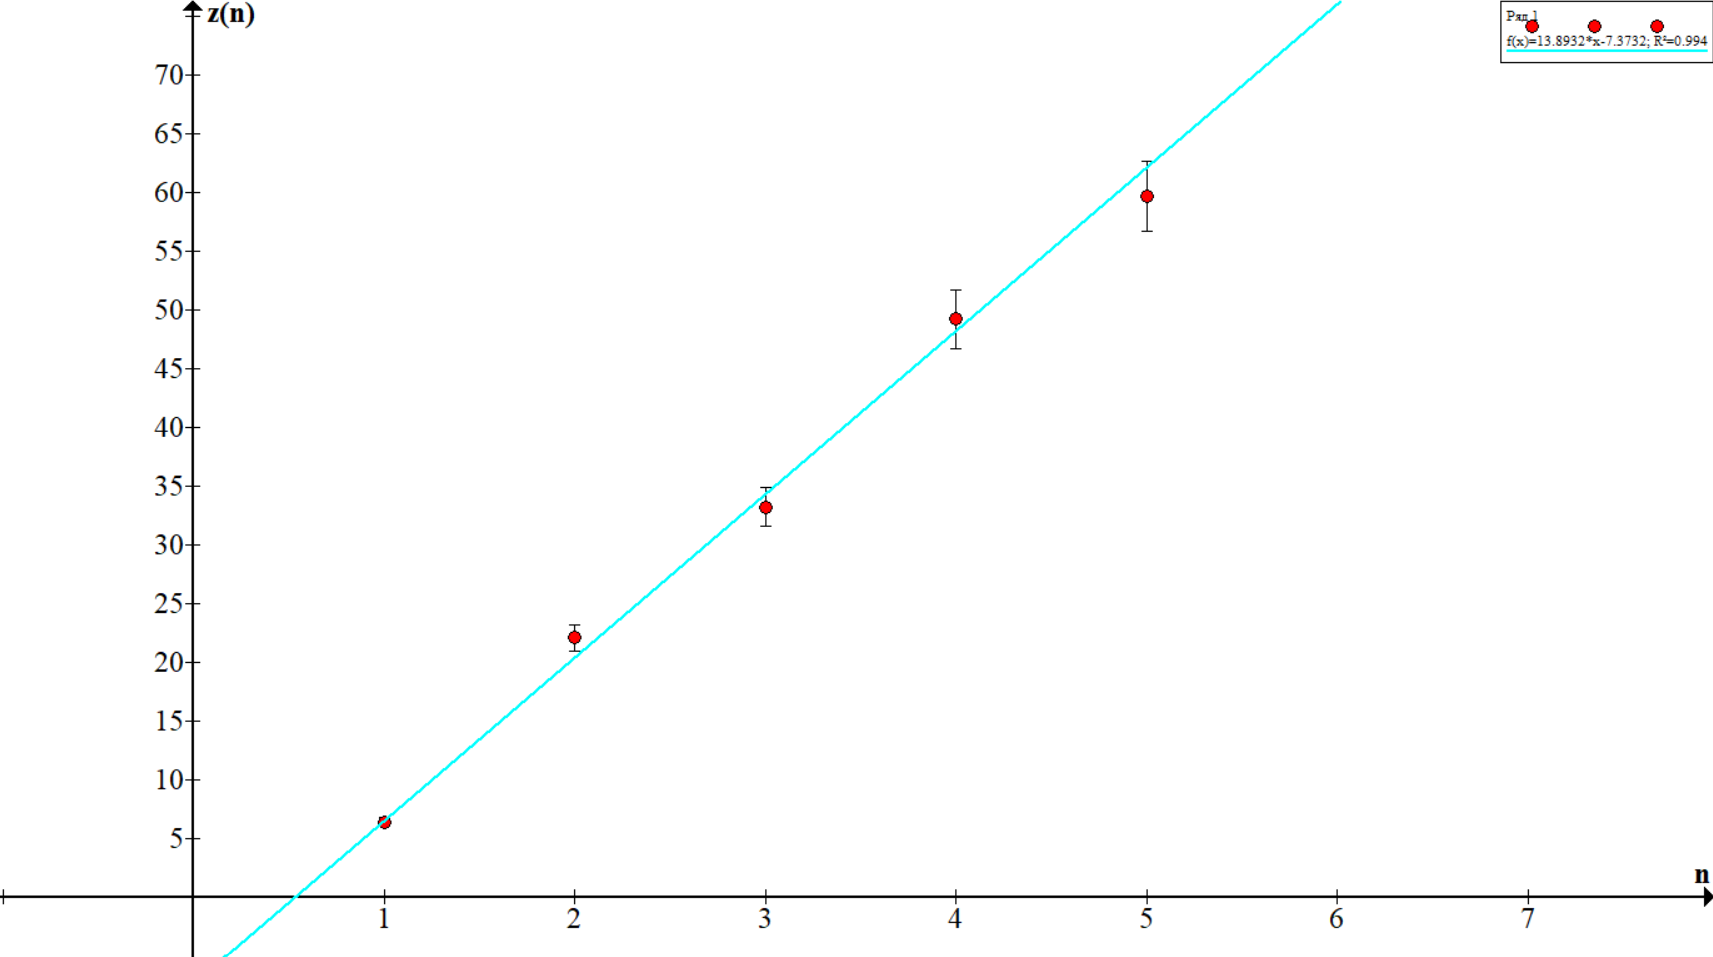
\includegraphics[width=13cm]{pics/lab_436_3.png}
  \caption{График $z_3 = f(n)$}
  \label{}
\end{figure}


\begin{figure}[h!]
  \centering
  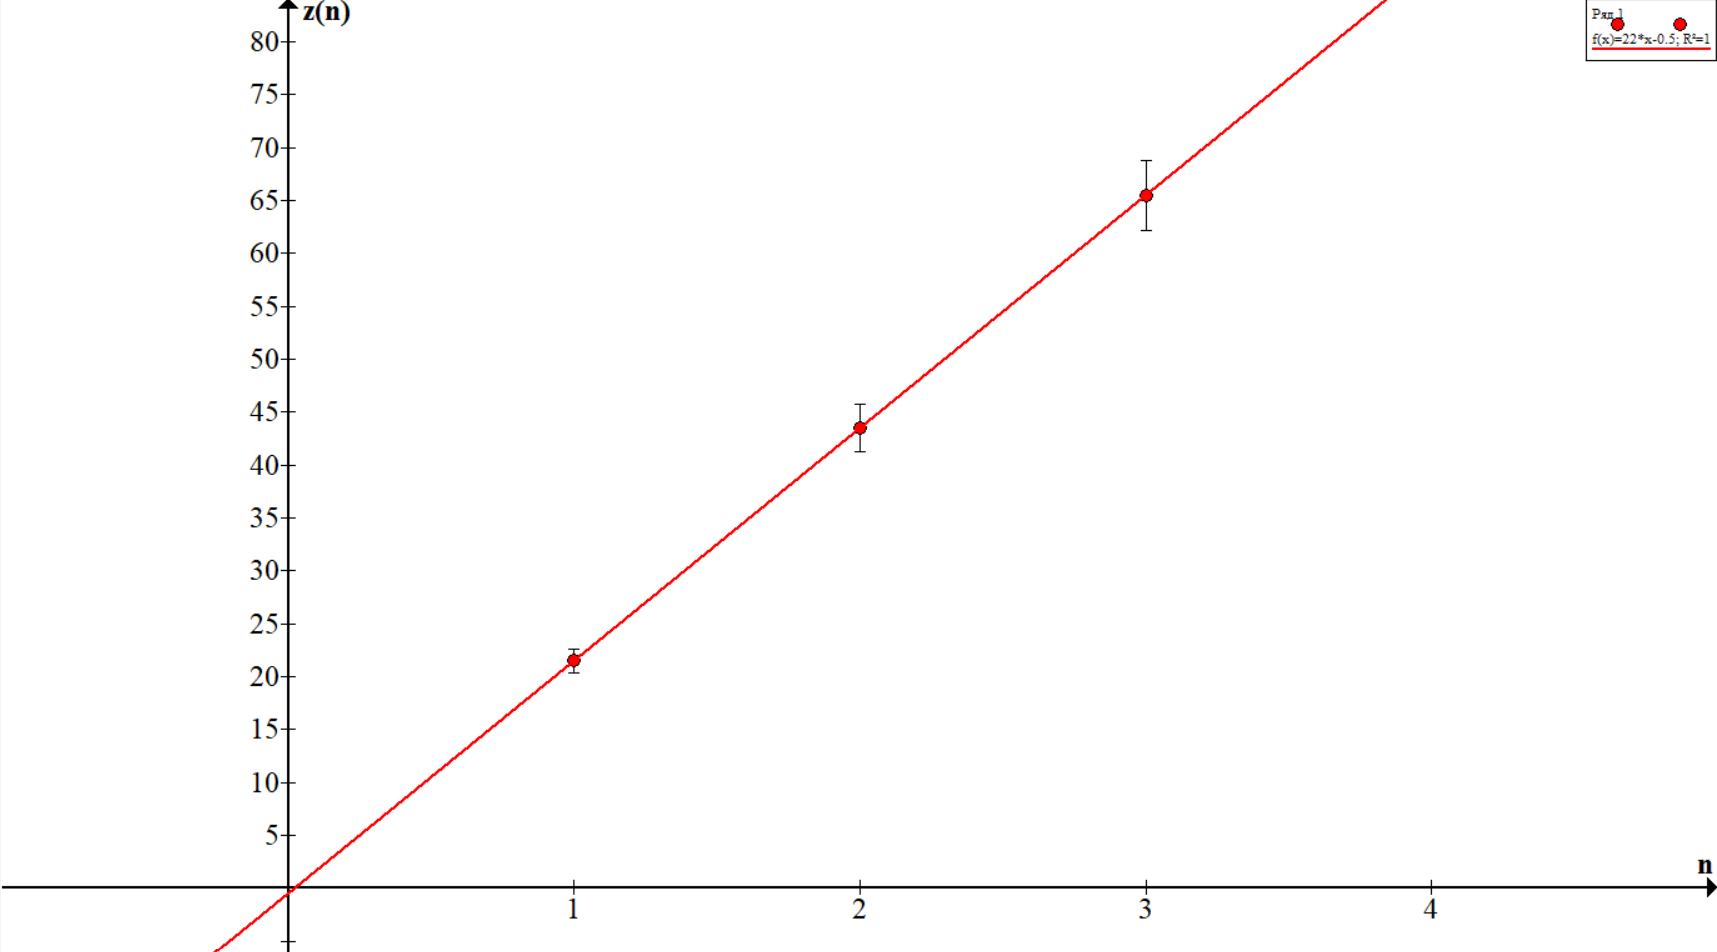
\includegraphics[width=13cm]{pics/lab_436_4.png}
  \caption{График $z_4 = f(n)$}
  \label{}
\end{figure}


\subsection{Исследование миры}

Измеряем расстояние между экраном и линзой - $L_3$, экраном и мирой - $L_4$.
Получаем, что $L_3 = 126 cm$, $L_4 = 132 cm$.

Ширина штриха миры равна $1 mm$.




\begin{table}[h!]
	\centering
	\begin{tabular}{| c | c | c |}
\hline
$n$ & $z_n (25), mm$ & $z_n (20), mm$\\
\hline
-3 & 17 & 12,2\\
\hline
-2 & 20 & 17,2\\
\hline
-1 & 23 & 22,5\\
\hline
0 & 26,1 & 28\\
\hline
1 & 28,3 & 33\\
\hline
2 & 31,9 & 38\\
\hline
3 & 34,5 & 43,5\\
\hline
4 & 37,5 & 48,5\\
\hline
5 & 41,1 & -\\
\hline
\end{tabular}

	\caption{Исследование решеток миры}
	\label{tb2_1}
\end{table}

\end{document}